
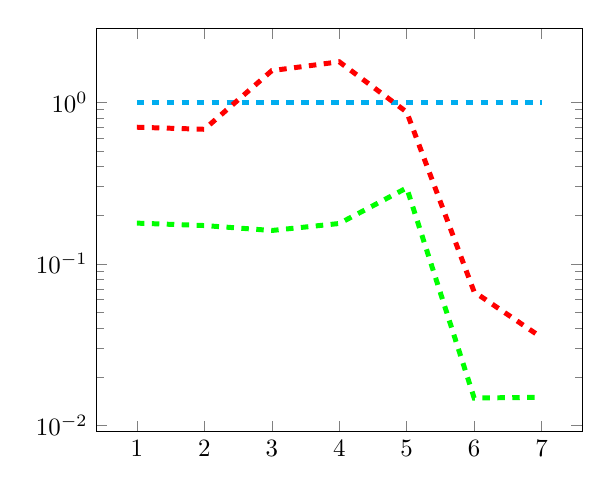
\begin{tikzpicture}[scale=0.9]
\begin{semilogyaxis}
\addplot[dashed,color=cyan,line width=2pt] coordinates {(1,1.0)(2,1.0)(3,1.0)(4,1.0)(5,1.0)(6,1.0)(7,1.0)};
\addplot[dashed,color=red,line width=2pt] coordinates {(1,0.6991711491790592)(2,0.678979386634632)(3,1.565408538881175)(4,1.7753063700081448)(5,0.867344241117009)(6,0.06700968889927464)(7,0.03498535434151886)};
\addplot[dashed,color=green,line width=2pt] coordinates {(1,0.1784520862382028)(2,0.17242030023807006)(3,0.16067863792748313)(4,0.17752907003388038)(5,0.29466787731606814)(6,0.014786794141857294)(7,0.014944567203630698)};

\end{semilogyaxis}
\end{tikzpicture}
